\documentclass{article}
\usepackage[UTF8]{ctex}
% Replace `letterpaper' with`a4paper' for UK/EU standard size
\usepackage[a4paper,top=2cm,bottom=2cm,left=3cm,right=3cm,marginparwidth=1.75cm]{geometry}

% Useful packages
\usepackage{amsmath}
\usepackage{graphicx}
\usepackage[colorlinks=true, allcolors=blue]{hyperref}
\usepackage{graphicx} %插入图片的宏包
\usepackage{float} %设置图片浮动位置的宏包
\usepackage{subfigure} %插入多图时用子图显示的宏包
\usepackage{parskip}
\usepackage{indentfirst} 
\setlength{\parindent}{2em}
\usepackage{hyperref}  
\usepackage{tikz}
\allowdisplaybreaks
\usepackage{multirow}
\usepackage{amsmath}
\usepackage{amsfonts,amssymb} 
\usepackage{xcolor} % 用于显示颜色
\usepackage{listings} % 用于插入代码
\lstset{
	basicstyle          =   \sffamily,          % 基本代码风格
	keywordstyle        =   \bfseries,          % 关键字风格
	commentstyle        =   \rmfamily\itshape,  % 注释的风格,斜体
	stringstyle         =   \ttfamily,  % 字符串风格
	flexiblecolumns,                % 别问为什么,加上这个
	numbers             =   left,   % 行号的位置在左边
	showspaces          =   false,  % 是否显示空格,显示了有点乱,所以不现实了
	numberstyle         =   \zihao{-5}\ttfamily,    % 行号的样式,小五号,tt等宽字体
	showstringspaces    =   false,
	captionpos          =   t,      % 这段代码的名字所呈现的位置,t指的是top上面
	frame               =   lrtb,   % 显示边框
}

\lstdefinestyle{Python}{
	language        =   Python, % 语言选Python
	basicstyle      =   \zihao{-5}\ttfamily,
	numberstyle     =   \zihao{-5}\ttfamily,
	keywordstyle    =   \color{blue},
	keywordstyle    =   [2] \color{teal},
	stringstyle     =   \color{magenta},
	commentstyle    =   \color{red}\ttfamily,
	breaklines      =   true,   % 自动换行,建议不要写太长的行
	columns         =   fixed,  % 如果不加这一句,字间距就不固定,很丑,必须加
	basewidth       =   0.5em,
}

\title{图像处理第1次作业报告}
\author{林子开}

\begin{document}
	\maketitle
	\tableofcontents

\section{Contrast stretching by piecewise linear transformation}
\subsection{python codes}
The python codes of exercise 1 are as follows:
\lstinputlisting[style = Python,
caption={The python codes for piecewise linear transformation},
label = {PLT}]{exercise1.py}
\par The function piecewise$\_$transf is called to perform piecewise linear transformation on the intensity of the intensity of each pixel.

\subsection{test example}
Now we shall test the codes above with the following transformation:
\[
f(x) =
\begin{cases}
x &\quad\text{if } x<5\\
5 + \frac{(x-5)(80-5)}{40-5} &\quad\text{if } 5\le x \le 40 \\
80 + \frac{(x-40)(255-80)}{255-40} &\quad\text{if } x > 40\\
\end{cases}
\]

\par Here is the comparison between the original figure and the transformed figure.


\begin{figure}[H]
	\centering
	\subfigure[the original figure]
	{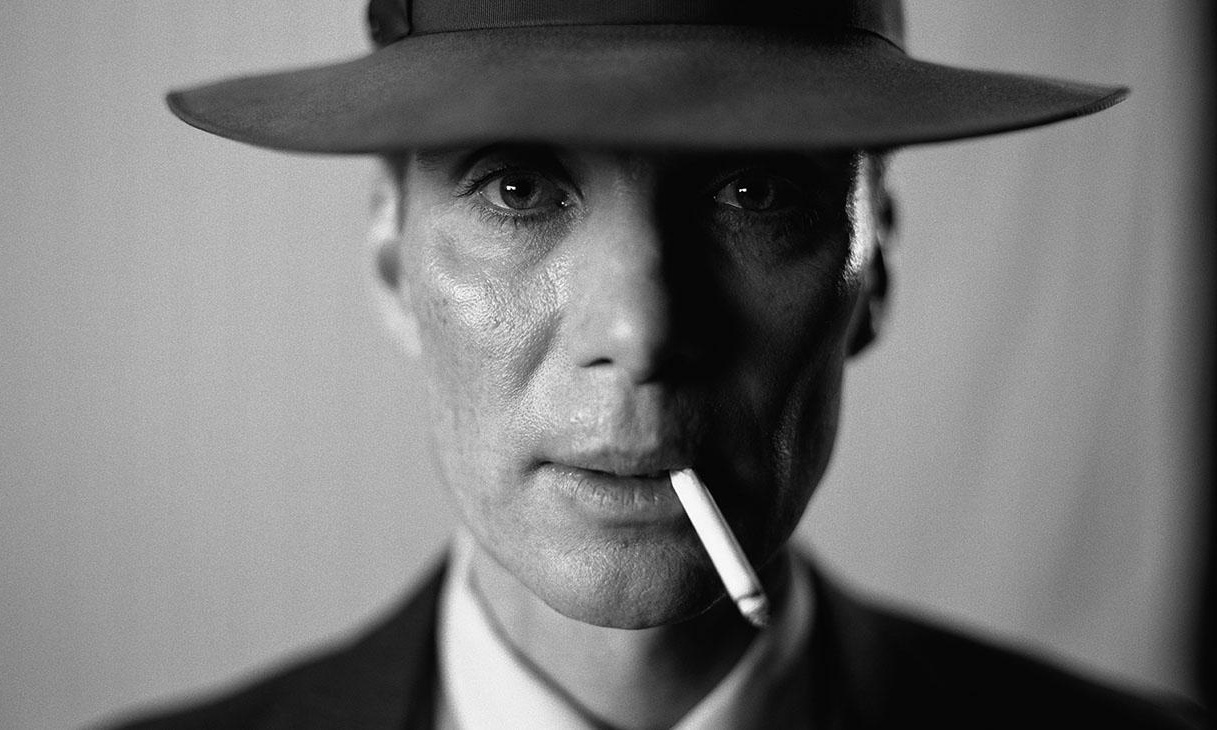
\includegraphics[width=0.45\textwidth]{image//test1.jpeg}}\label{ob}
	\,    % 重点就在这,优先横向排列,自动换行
	\subfigure[the transformed figure]
	{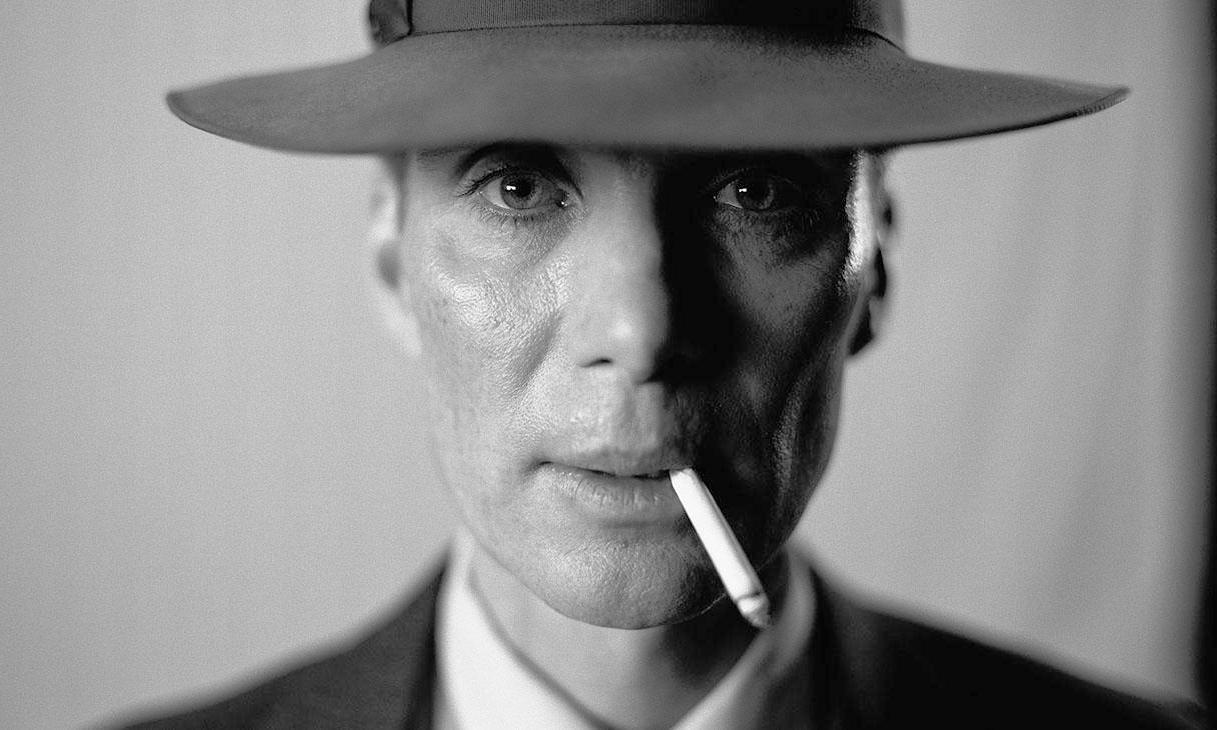
\includegraphics[width=0.45\textwidth]{image//piecewise linear transformation fortest1.jpeg}}\label{ob_trans}
	\caption{the comparison between the original figure and the transformed figure in exercise 1}
\end{figure}

It can be observed that the contrast is stretched after the piecewise linear transformation
especially for the darker half of the man's face.




\section{Computation of joint histogram}

\subsection{Global n-dimension joint histogram}
\subsubsection{python codes}
    The core function is as follows:
        \lstinputlisting[style = Python,
        caption={The core python codes for n-dimension joint histgoram},
        label = {extra-max},
        linerange={12-36}]{exercise2_1.py} 
    This function visit every element in the data, get the values in each dimension of the element,
    and add the tuple of values to the n-dimension joint histogram with bins given.
 
\subsubsection{test example: 2-dimension joint histgoram}
Here I test the codes above by a 2-dimension data. This data consists of 
red levels and green levels corresponding to every pixel from the following test figure:
\begin{figure}[H]
    \centering  %图片全局居中
    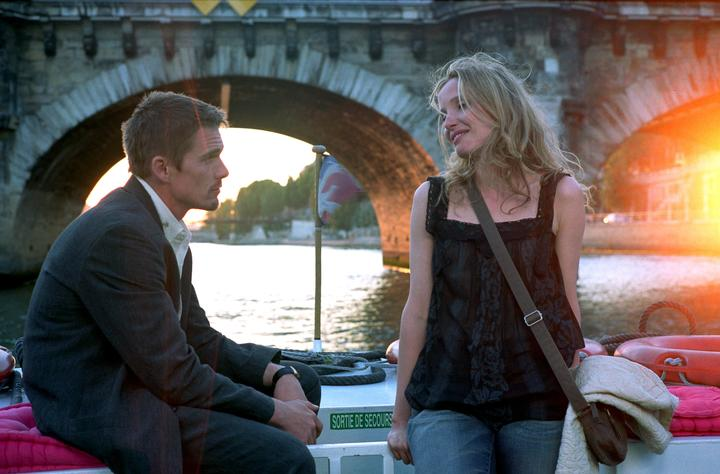
\includegraphics[width=0.5\textwidth]{image//test2.jpg}
    \caption{the colored figure for test in exercise 2}
\end{figure}
I set bins=256 for the two dimensions and the results are as follows:
\begin{figure}[H]
	\centering
	\subfigure[the 2-D histogram]
	{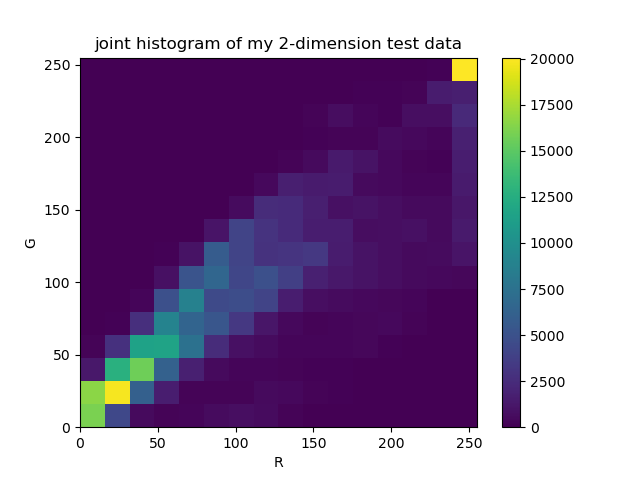
\includegraphics[width=0.49\textwidth]{image//test2_2d_colorful_histogram.png}}
	\,    % 重点就在这,优先横向排列,自动换行
	\subfigure[the 3-D histogram]
	{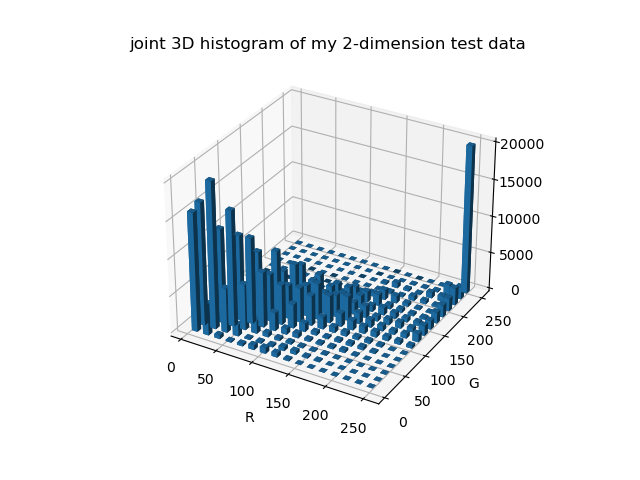
\includegraphics[width=0.49\textwidth]{image//test2_3d_bar.png}}
	\caption{the joint histogram of the red levels and the green levels of every pixel from test figure}
\end{figure}


\subsection{Local 2-dimension joint histogram}
\subsubsection{python code}

The core function for efficiently computing the local histogram of an image is as follows:
    \lstinputlisting[style = Python,
    caption={The core python codes for efficient local joint histgoram computation},
    label = {efficient},
    linerange={17-60}]{exercise2_2.py} 

    This function updating the local histogram with the new column introduced
    and the old column abandoned in a motion step.
\subsubsection{test example}
    I test the codes on the original figure\ref{ob} from exercise 1.
    Since there are too many local histogram, I've seleced three groups 
    of neighboured ones. They are the first 3, the middle 3, and the last 3 local histograms.
    
    I set the patch size 25*25, and here are the results:
        \begin{figure}[H]
        \centering
        \subfigure[centered at (0,0)]
        {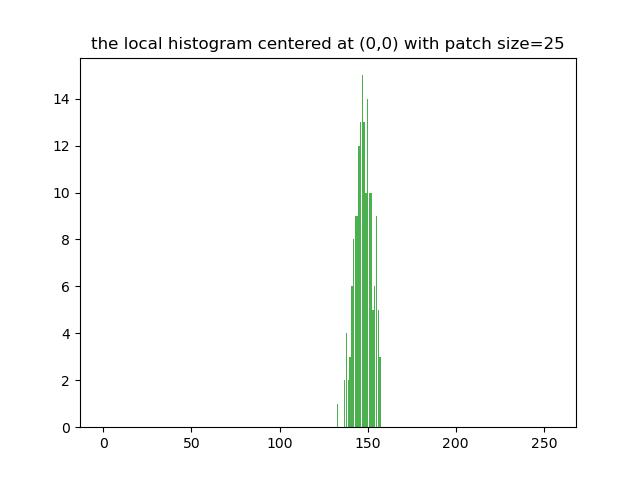
\includegraphics[width=0.3\textwidth]{image//the local histogram centered at (0,0) with patch size=25.jpg}}
        \,  
        \subfigure[centered at (0,1)]
        {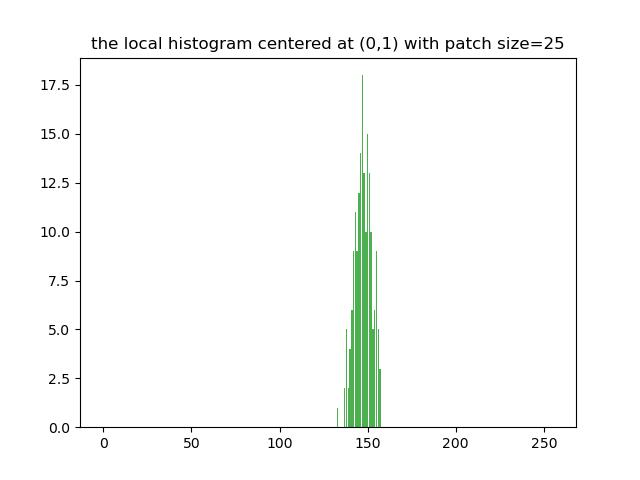
\includegraphics[width=0.3\textwidth]{image//the local histogram centered at (0,1) with patch size=25.jpg}}
        \,  
        \subfigure[centered at (0,2)]
        {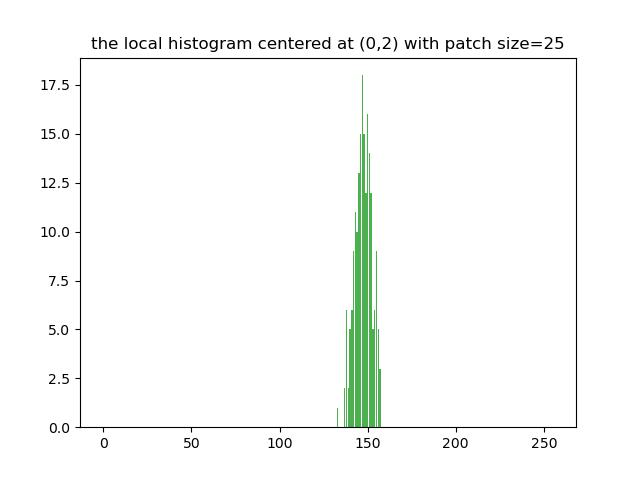
\includegraphics[width=0.3\textwidth]{image//the local histogram centered at (0,2) with patch size=25.jpg}}
        \,  
        \subfigure[centered at (365,20)]
        {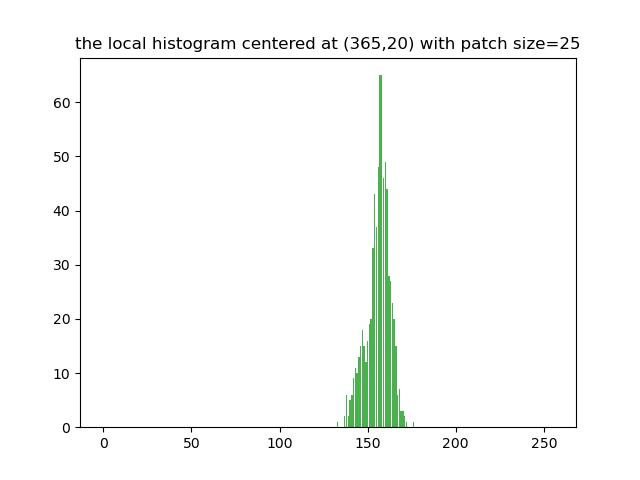
\includegraphics[width=0.3\textwidth]{image//the local histogram centered at (365,20) with patch size=25.jpg}}
        \,  
        \subfigure[centered at (365,21)]
        {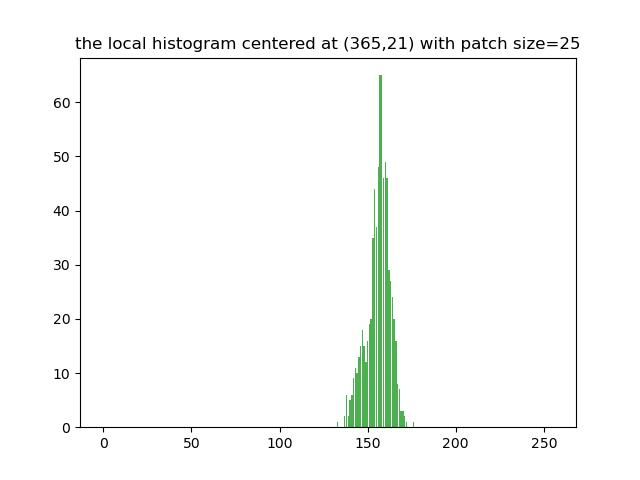
\includegraphics[width=0.3\textwidth]{image//the local histogram centered at (365,21) with patch size=25.jpg}}
        \,  
        \subfigure[centered at (365,22)]
        {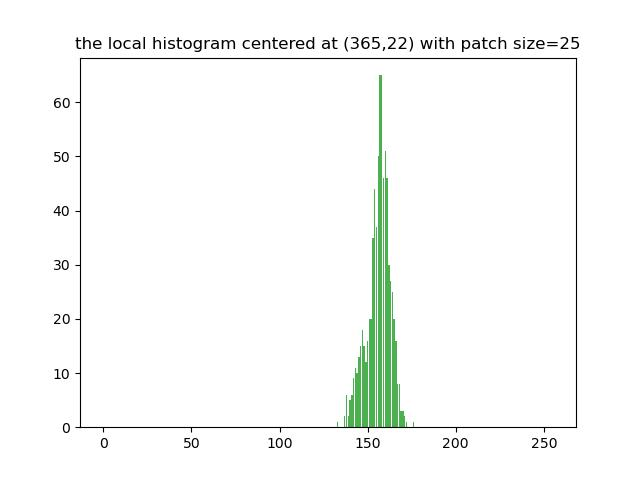
\includegraphics[width=0.3\textwidth]{image//the local histogram centered at (365,22) with patch size=25.jpg}}
        \,  
        \subfigure[centered at (729,1214)]
        {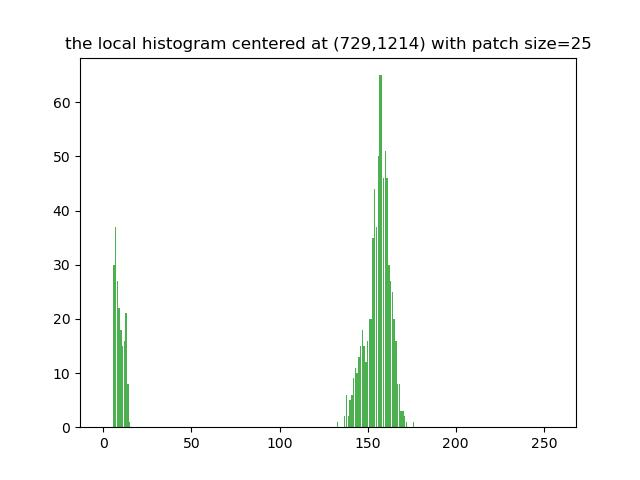
\includegraphics[width=0.3\textwidth]{image//the local histogram centered at (729,1214) with patch size=25.jpg}}
        \,  
        \subfigure[centered at (729,1215)]
        {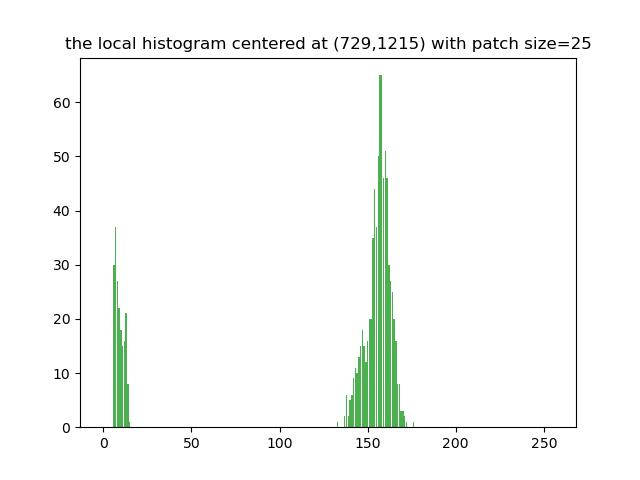
\includegraphics[width=0.3\textwidth]{image//the local histogram centered at (729,1215) with patch size=25.jpg}}
        \,  
        \subfigure[centered at (729,1216)]
        {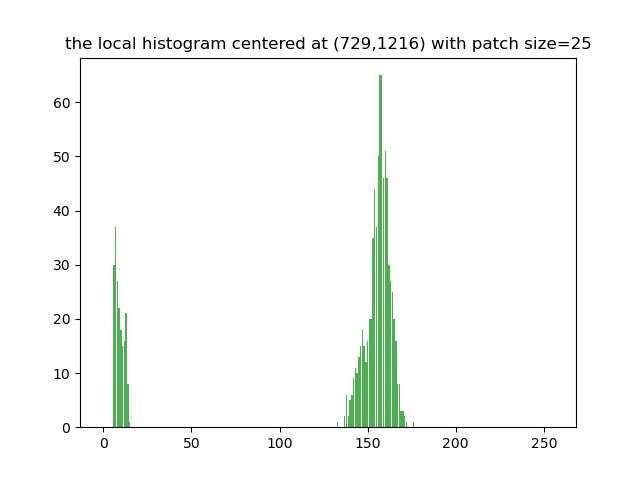
\includegraphics[width=0.3\textwidth]{image//the local histogram centered at (729,1216) with patch size=25.jpg}}
        \,
        \caption{some of the neighboured local histograms}
        \end{figure}


\section{Histgoram equalization}
\subsection{Global equalization}
\subsubsection{python codes}
    The core python codes for global equalization are as follows:
    \lstinputlisting[style = Python,
    caption={The core python codes for global equalization},
    label = {efficient},
    linerange={59-108}]{exercise3.py} 
    
    The codes above first generate the global histgoram of the figure.
    Based on the global histgora, a list is computed to map from the intensity in the original
    figure to that in the globally equalized figure.
\subsubsection{test example}
    Here I select a gray figure under electronic microscope. To enhance its contrast, 
    first perform global equalization on it. The comparison is as follows:
    \begin{figure}[H]
        \centering
        \subfigure[the original figure]
        {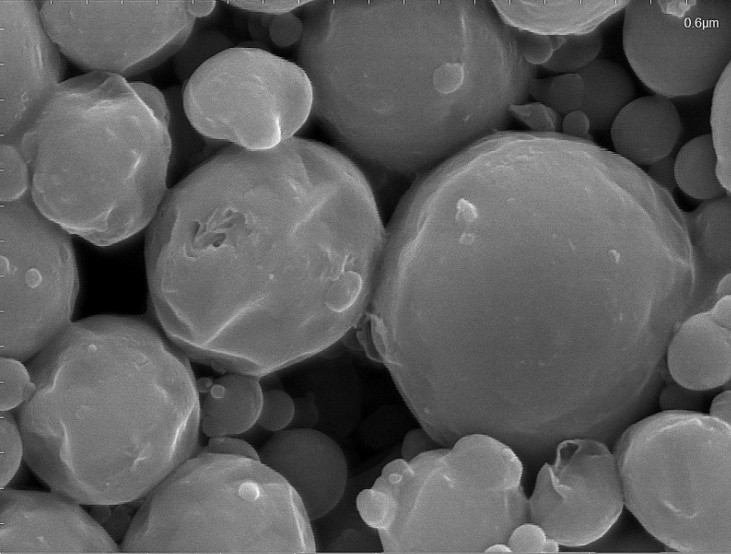
\includegraphics[width=0.49\textwidth]{image//test3.png}}\label{elec}
        \,    % 重点就在这,优先横向排列,自动换行
        \subfigure[the globally equalized figure]
        {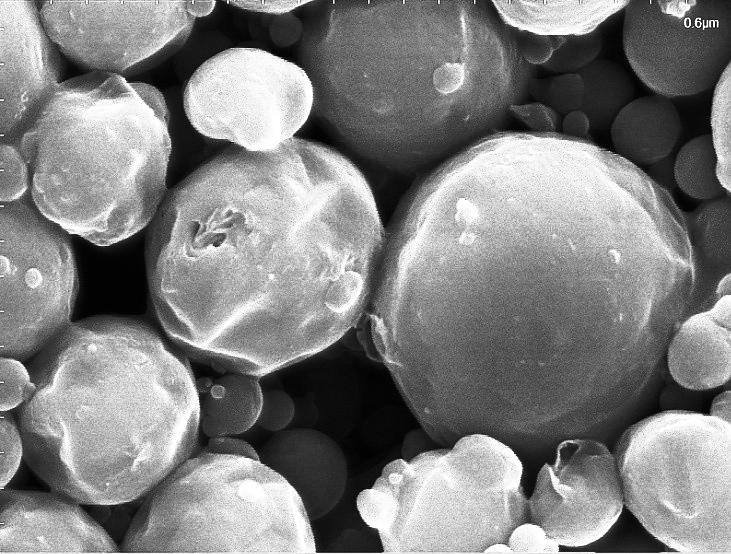
\includegraphics[width=0.49\textwidth]{image//global equalization.jpg}}
        \caption{the orignal figure compared with the globally equalized figure}
    \end{figure}

\subsection{Local equalization}
\subsubsection{python codes}
The core python codes are as follows:
\lstinputlisting[style = Python,
caption={The core python codes for local equalization},
label = {efficient},
linerange={110-125}]{exercise3.py} 

The local$\_$hist function is the same as that in exercise 2, 
so we shall omit the details of it.

For local equalization, we still generate the local histograms corresponding to every pixel.
Based on the local histogram, we can perform the equalization transformation 
on the centered pixel. After that, we move to its neighboured one.
\subsubsection{test exaple}
I test the local equalization on orgianl figure\ref{elec} with different patch sizes of 
11, 51, 151, and 201. The results are as follows:
\begin{figure}[H]
    \centering
    \subfigure[patch size = 11]
    {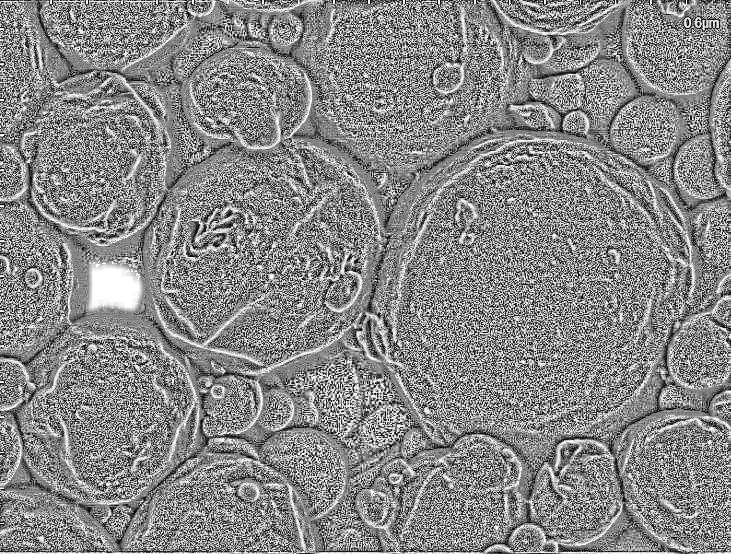
\includegraphics[width=0.49\textwidth]{image//local equalization with patch size = 11.jpg}}
    \,    % 重点就在这,优先横向排列,自动换行
    \subfigure[patch size = 51]
    {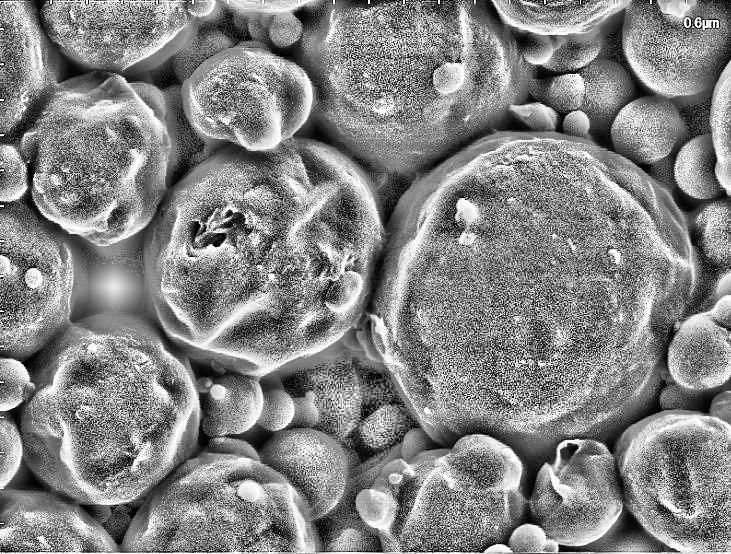
\includegraphics[width=0.49\textwidth]{image//local equalization with patch size = 51.jpg}}
    \,
    \subfigure[patch size = 151]
    {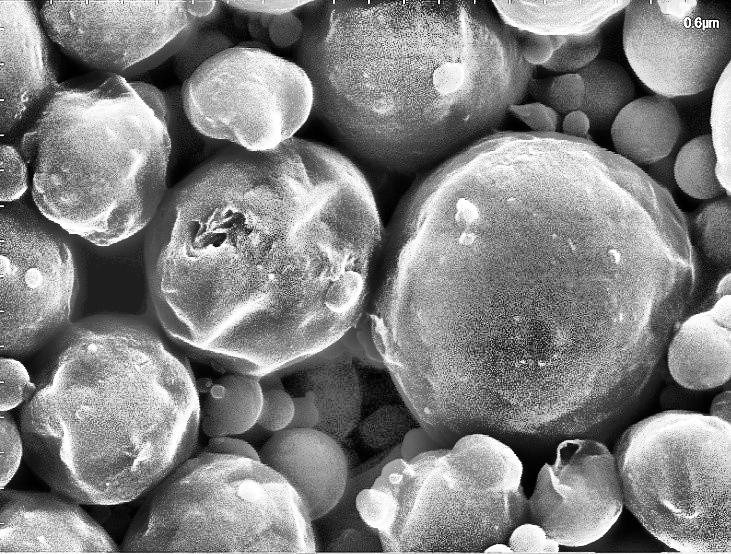
\includegraphics[width=0.49\textwidth]{image//local equalization with patch size = 151.jpg}}
    \,    % 重点就在这,优先横向排列,自动换行
    \subfigure[patch size = 201]
    {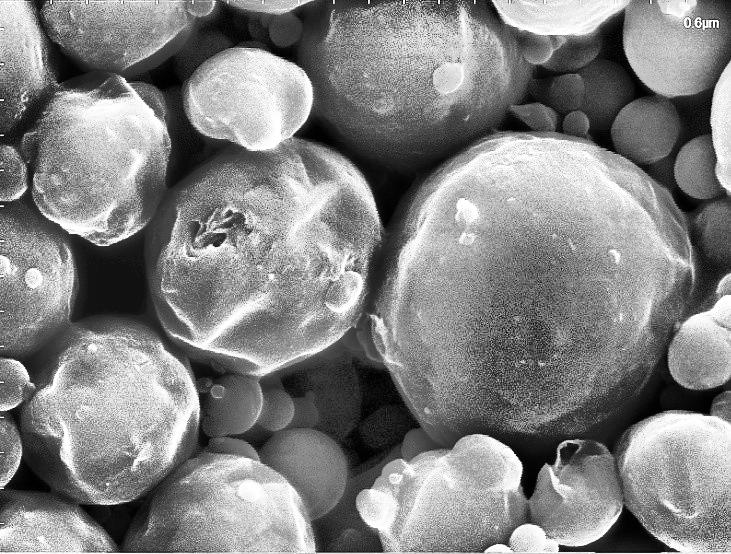
\includegraphics[width=0.49\textwidth]{image//local equalization with patch size = 201.jpg}}
    \caption{local equalization with different patch sizes}
\end{figure}


It seems that the local equalization with patch size=151 can 
show the best details among the four patch sizes. 

% \lstinputlisting[style = Python,
% caption={The implementation of EXTRA-MAX},
% label = {extra-max},
% linerange={33-55}]{d_ary_heap.py} 

% \begin{figure}[H]
%     \centering  %图片全局居中
%     \includegraphics[width=0.8\textwidth]{result3}
%     \caption{The heap after performing INCREASE-KEY(A, 10, 28)}
% \end{figure}

% \begin{figure}[htbp]
% 	\centering
% 	\subfigure[扰动=0.1]
% 	{\includegraphics[width=0.45\textwidth]{八字形轨道-初值敏感1//扰动=0.1}\label{8_orbit_error_1e-1}}
% 	\,    % 重点就在这,优先横向排列,自动换行
% 	\subfigure[扰动=0.01]
% 	{\includegraphics[width=0.45\textwidth]{八字形轨道-初值敏感1//扰动=0.01}\label{8_orbit_error_1e-2}}
% 	\,
% 	\subfigure[扰动=0.001]
% 	{\includegraphics[width=0.45\textwidth]{八字形轨道-初值敏感1//扰动=0.001}\label{8_orbit_error_1e-3}}
% 	\,
% 	\subfigure[扰动=0.0001]
% 	{\includegraphics[width=0.45\textwidth]{八字形轨道-初值敏感1//扰动=0.0001}\label{8_orbit_error_1e-4}}
	
% 	\caption{"8"字形轨道的初值受到不同程度扰动后的突变情况,$t\in[0,200]$}
% \end{figure}

\end{document}